\chapter{Experiments}\label{chapter:experiments}

In this chapter, we study and experiment with the training method we introduced
in Chapter~\ref{chapter:training_method}. While the main goal of this chapter
is to outperform both teacher models and the base student checkpoint, we also
want to show that each teacher contributes to the student's performance.

This chapter is laid out as follows. First we describe the training data in
Section~\ref{section:val_training_data}. Second we discuss how we compare
models in Section~\ref{section:validation_tasks}. Third we present the
student's configuration and define the baselines in
Section~\ref{section:student_model_config_baselines}. Then we experiment with
the structural loss in Section~\ref{section:structural_loss}. With the
structural loss already given, we find the best performing contextual loss and
the weighting of the two losses in Section~\ref{section:improving_both}.

\section{Training data}\label{section:val_training_data}

We create the training dataset for our validation, labelled as
\Dataset{val\_500k}, similarly to how we put together the final training
dataset \Dataset{train\_1500k} in Chapter~\ref{chapter:evaluation}. In short,
we equally sample documents from English Wikipedia and RealNews articles
\citep{zellers2019defending}, which are at least 1200 Longformer tokens long.
We use a subset of Longormer's training data, to make the comparison between a
learned student model and its base checkpoint fair. In this way, the trained
student model will not see any new data compared to Longformer. Thus any
performance gains of the student model over its base checkpoint, can be
attributed to our training method, rather than to a higher-quality training
dataset.

We show some of the statistics of \Dataset{val\_500k} in
Table~\ref{table:val_data_stats}. Very similar to \Dataset{train\_1500k},
\Dataset{val\_500k} contains long documents that are, on average, over 1300
tokens long. Consequently only about 34\% of the documents could be processed
whole using a traditional Transformer such as RoBERTa \citep{liu2019roberta} or
SBERT. We also display document's length distribution in
Figure~\ref{fig:val_data_dist}. As Wikipedia contains relatively short documents,
while RealNews does not contain document below 1200 tokens, the source's
distributions are well spaced out.


\begin{table}
  \centering
  \footnotesize

  \begin{tabular}{lrr}
    \toprule
      Split & Train & Validation \\
    \midrule
      Documents & 500 000 & 10 000 \\
      Tokens & 6.85e+08 & 1.37e+07 \\
      Tokens per document & 1370.74$\pm$1723.38 & 1371.65$\pm$1717.24 \\
      SBERT tokens over 384 & 70.56\% & 70.07\% \\
      SBERT tokens over 512 & 66.37\% & 66.14\% \\
    \bottomrule
  \end{tabular}

  \caption{Statistics of \Dataset{val\_500k}. For each split we also show the
  percentage of documents with the number of SBERT tokens above given
  threshold.}

  \label{table:val_data_stats}

\end{table}

\begin{figure}

  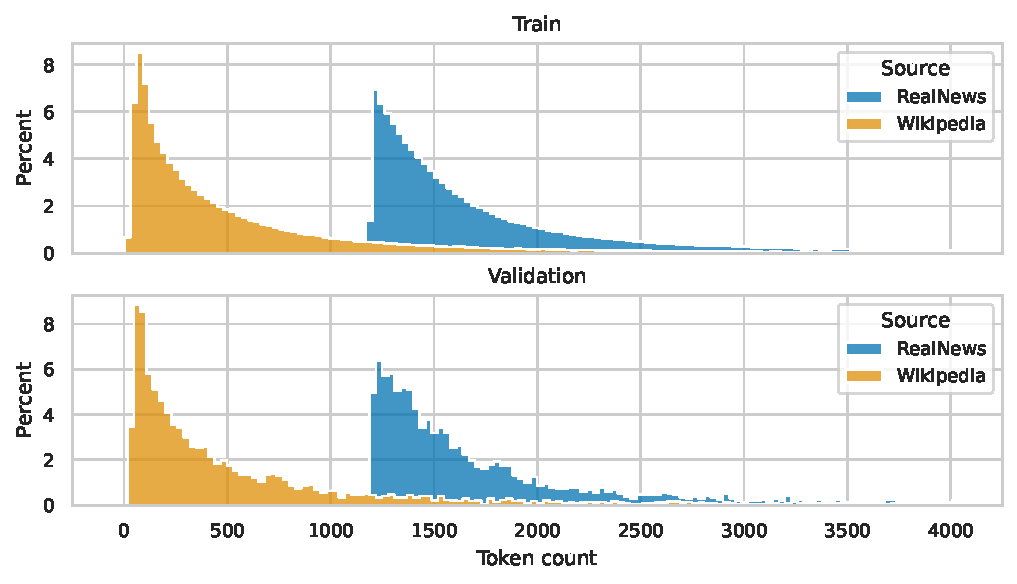
\includegraphics[width=\textwidth]{./img/val_data_dist.pdf}

  \caption{Distribution of train and validation documents' lengths for
  \Dataset{val\_500k}.}

  \label{fig:val_data_dist}

\end{figure}

\section{Validation tasks}\label{section:validation_tasks}

We compare the embedding models based on their performance on a set of
downstream tasks. We use a subset of our evaluation tasks, which we describe in
Chapter~\ref{chapter:evaluation}. We include tasks that either have large
enough training split suitable for cross-validation or a validation split. All
tasks are classifications that are evaluated using a validation split, except
for \Task{IMDB}, where we take the mean score of five cross-validation folds.
To make the validation faster to compute we downsample the validation and train
splits to 10000 examples. We downsample the datasets according to their label
distribution, so that the truncated split has nearly identical label
distribution to the original one. We present the validation tasks along with
their document count in Table~\ref{table:validation_tasks}.

We use binary or micro-averaged accuracy as the scoring metric. Often we need to
compare performance across several tasks. However not all tasks are equally
difficult and so averaging accuracies would lead us to favoring models that
performed well on easy tasks, and undervaluing models that performed well on the
more difficult tasks. Therefore, we normalize the accuracy by the highest score
reached for the given task within the considered models and thereby making the
tasks equally difficult. We call this metric \emph{normalized accuracy}.

When validating a trained embedding model on a task we finetune a head that
transforms the embeddings into the output format required by the given task. We
do not finetune the embedding model itself. Besides speeding up the validation,
this gives us also more genuine picture of the performance of the embedding
model. Since all our validation tasks are classifications, the heads are just
2-layer neural network classifiers with a cross-entropy loss. We present the
complete list of classifier's hyperparameters and training parameters in
Table~\ref{table:head_train_params}.

\begin{table}
  \footnotesize
  \centering
  \begin{tabular}{llrrrr}
    \toprule
      & \multicolumn{2}{c}{Documents} & Classes & \multicolumn{2}{c}{Class percentage} \\
    \cline{2-3} \cline{5-6}
      Dataset & Train & Test & & Train & Validation \\
    \midrule
      \Task{arxiv} \citep{arxiv_papers} & \dag10 000 & 2 500 & 11 & 9.09$\pm$1.24\% & 9.09$\pm$1.01\% \\
      \Task{imdb} \citep{maas2011learning} & \dag10 000 & - & 2 & 50.00$\pm$0.00\% & - \\
      \Task{oc} \citep{zhou2020multilevel} & \dag10 000 & \dag10 000 & 2 & 50.00$\pm$0.06\% & 50.00$\pm$0.15\% \\
      \Task{aan} \citep{zhou2020multilevel} & \dag10 000 & \dag10 000 & 2 & 50.00$\pm$1.50\% & 50.00$\pm$4.57\% \\
      \Task{s2orc} \citep{zhou2020multilevel} & \dag10 000 & \dag10 000 & 2 & 50.00$\pm$0.09\% & 50.00$\pm$0.32\% \\
      \Task{pan} \citep{zhou2020multilevel} & \dag10 000 & 2 908 & 2 & 50.00$\pm$0.00\% & 50.00$\pm$0.00\% \\
    \bottomrule
  \end{tabular}

  \caption{Validation tasks we use for comparing embedding models in this
  chapter. We truncated splits marked with {\dag} to speed up validation of
  models. We truncate a split by downsampling it according to its label
  distribution. The class distributions of all tasks are well balanced except
  for \Task{aan} as can be seen from the mean and standard deviation of class
  percentages for given task and split.}

  \label{table:validation_tasks}

\end{table}


\begin{table}
  \centering
  \footnotesize

  \begin{tabular}{l c}
    \toprule
    Parameter & Value \\
    \midrule
    Hidden features & 50 \\
    Hidden dropout rate & 0.5 \\
    Hidden activation & ReLU \\
    Epochs & 10 \\
    Batch size & 32 \\
    Weight decay & 0.1 \\
    Label smoothing & 0.1 \\
    Learning rate & 1e-4 \\
    Learning rate decay & Cosine \\
    Maximum gradient norm & 1.0 \\
    Optimizer & AdamW \\
    Mixed-precision training & Yes \\
    \bottomrule
  \end{tabular}

  \caption{Training hyperparameters used for training classification heads
  during validation.}

  \label{table:head_train_params}

\end{table}

\section{Student's model configuration and baselines}\label{section:student_model_config_baselines}

As we explained in Section~\ref{section:student_model}, we chose
Longformer \citep{beltagy2020longformer} as our student model. We use
Longformer's base version with about 126M parameters implemented by
HuggingFace \texttt{transformers}
library\footnote{\url{https://huggingface.co/allenai/longformer-base-4096}}.

To obtain the input's embedding we average the last layer's hidden states. We
do not use global attention and restricting ourselves to only sliding window
attention, with the window sizes $\omega$ set to the default 512 tokens. We
also experimented with obtaining the document embedding from the last layer's
hidden state of the \texttt{[CLS]} token, while simultaneously setting the
global attention for the same token. However, this configuration resulted in
worse performance and thus we continue using mean pooling of the last layer's
hidden states and no global attention.

During training of the student model we aim for fast convergence with small
memory footprint. We therefore use high learning rate, no gradient accumulation
steps, mixed-precision training and gradient checkpointing. We enumerate the
complete list of used training parameters' values in
Table~\ref{table:student_train_params}, which we use in all student's
trainings.


\begin{table}
  \centering
  \footnotesize

  \begin{tabular}{l c}
    \toprule
    Parameter & Value \\
    \midrule
    Batch size & 6 \\
    Weight decay & 0.1 \\
    Learning rate & 1e-4 \\
    Learning rate decay & Cosine \\
    Maximum gradient norm & 1.0 \\
    Optimizer & AdamW \\
    Gradient accumulation steps & 1 \\
    Warmup steps & 10\% of training steps \\
    Gradient checkpointing & Yes \\
    Mixed-precision training & Yes \\
    \bottomrule
  \end{tabular}

  \caption{Training parameters' values used for all student's trainings in this
  chapter.}

  \label{table:student_train_params}

\end{table}

\subsection{Baselines}

As we already mentioned in the beginning of this chapter, the goal of the
following experiments is to surpass both teachers as well as the base
checkpoint of our student model using our teacher-student training approach. To
that end we compare our student model throughout this chapter to three models:
Longformer \citep{beltagy2020longformer}, SBERT \citep{reimers2019sentence},
and PV \citep{le2014distributed}. Longformer is the base checkpoint of our
student model. By comparing the student model to Longformer, we judge how much
our training method improves document embeddings. As we mentioned above, we use
a subset of Longformer pre-training data to eliminate the option that the
student model gains performance just because of the new training data. For
context, we train the student models for only 3.8\% iterations of Longformer's
pre-training with 8-times smaller batch size.

We compare the student models to the two teachers; SBERT and PV. We hope to
surpass both teachers by combining their respective qualities and the
architectural advantages of the student model over the teachers. Compared to
SBERT, the student model has maximal context 8 times longer, whereas compared
to PV it has much more parameters and therefore should be able to learn more
complex structural relationships within the input. And so, by comparing the
student model to the teachers we estimate how well our method distills the
qualities of the teacher's embeddings into the student's. We discuss the
configuration and checkpoint of the structural teacher in the following
sections. Paragraph Vector's training is a part of our teacher-student training
method, and so we discuss further details in Section~\ref{section:pv_training},
where we experiment with PV's training hyperparameters. Until then we compare
the student model only to the structural teacher.

\section{Structural loss}\label{section:structural_loss}

We start our experiments with the structural loss $\Loss_S$. The structural
loss compares the student's and the structural teacher's embeddings and its
goal is to encourage distillation of the quality of the structural teacher's
embeddings into the student's embeddings. We focus on the structural loss first,
since in our preliminary experiments, we observed that the structural quality
is more essential to the performance of the student model than the contextual
quality. Note that we arrive to the same conclusions later in this chapter in
Section~\ref{section:projections_only_contextual}. Therefore, we prioritize
finding the best performing hyperparameters of the structural loss first and
adapting the contextual loss to it, after.

As we mention in Section~\ref{section:teacher_models}, we use SBERT
\citep{reimers2019sentence} as our structural teacher. We use SBERT's version
initialized with MPNet \citep{song2020mpnet}, since it is relatively small
model with above average
performance\footnote{\url{https://sbert.net/docs/pretrained_models.html}}. We
use SBERT's implementation from HuggingFace \texttt{transformers}
library\footnote{\url{https://huggingface.co/sentence-transformers/all-mpnet-base-v2}}
with mean pooling layer above the last layer's hidden states. We do not perform
any finetuning and use the pre-trained weights only.

As we explain in Section~\ref{section:abstract_loss}, we chose structural loss
to be more restrictive, forcing an exact similarity between the two embeddings.
Therefore, we try two different exact losses: Mean Squared Error (\emph{MSE})
and cosine distance. We chose MSE, because it forces equality -- the most
restrictive similarity measure. The motivation for using cosine comes from the
embeddings' use cases, where cosine distance is a popular similarity measure.
More importantly it is also used by SBERT's authors, suggesting that for
SBERT's embeddings, it is the best-performing similarity measure.

We train the student model with each loss on the first 15k documents of
\Dataset{val\_500k} with the hyperparameters given in
Section~\ref{section:student_model_config_baselines}. We compare the student's
performance to the relevant baselines: Longformer and SBERT. As we show in
Figure~\ref{fig:structural_basic}, with cosine distance the student model
manages to surpass both baselines. On the other hand, using MSE as a structural
loss has damaging effects on the student's performance. Notably, SBERT's scores
are significantly higher than Longformer's despite its much shorter context
length. That is to show, that unless the student's embeddings are finetuned,
its longer context length is of little benefit.

% This shows this can be useful training method in itself

To summarize, going forward we
use cosine loss as the structural loss.

\begin{figure}
  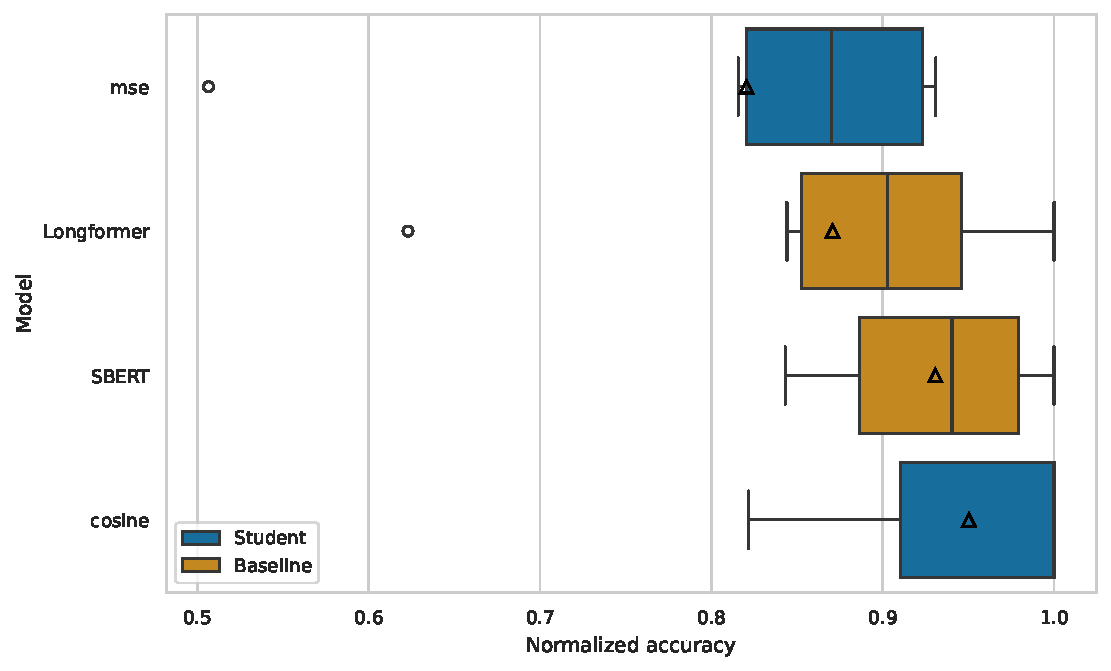
\includegraphics[width=\textwidth]{img/structural_simple_losses.pdf}

  \caption{Boxplot of normalized accuracies on validation tasks of baselines
  and student models trained with structural teacher. We mark the normalized
  accuracy means per model by a triangle.}

  \label{fig:structural_basic}
\end{figure}

\subsection{Composite structural losses}\label{section:composite_losses}

Besides the cosine and the MSE, we also explore losses that combine a positive
and a negative component, such as max-marginals or contrastive loss. We call
such losses \emph{composite} as opposed to the \emph{simple} losses, such as MSE
or cosine distance. In composite losses, the positive component compares the
student's and the corresponding teacher's embedding and rewards the model if
they are similar. The negative component compares the student's and the
non-corresponding teacher's embeddings and punishes the model if they are
similar. For brevity, we call the corresponding teacher's embedding
\emph{positive}, while the non-corresponding ones \emph{negatives}.

Our motivation behind the composite losses was that the negatives could give
the model a more precise indication where it should move its embeddings in the
vector space and therefore it could converge faster to the structural teacher's
embeddings. However, as we discuss in further subsections, this is not what
actually happens. Nevertheless, some of the models performed so well we do not
want to overlook these losses. Additionally, in our opinion, these experiments
are a solid ground for a future research.

We explored two types of composite losses: max-marginals and contrastive. Both
losses maximize the distance to the negatives while minimizing the distance to
the positive, but each does it differently, which is best shown by a formula.
We label the student's embedding as $y$, the corresponding teacher's embedding
as $y_{\text{pos}}$, the set of negatives as $Y_{\text{neg}}$, the given
similarity measure as $\operatorname{sim}$, and a weighting parameter as
$\gamma$. We formulate the max-marginals loss in
Equation~\ref{eq:max_marginals} and the contrastive loss in
Equation~\ref{eq:contrastive}.


\begin{equation}
  \Loss_{\text{max-marginals}}(y, y_\text{pos}, Y_\text{neg}) =
    \operatorname{sim}(y, y_\text{pos}) -
    \gamma \frac{1}{|Y_\text{neg}|} \sum_{y_\text{neg} \in Y_\text{neg}}
      \operatorname{sim}(y, y_\text{neg})
  \label{eq:max_marginals}
\end{equation}

\begin{equation}
  \Loss_{\text{contrastive}}(y, y_\text{pos}, Y_\text{neg}) =
    -\log \frac{
      \exp(\cos(y, y_\text{pos}))
    }{
      \exp(
        \cos(y, y_\text{pos}) +
        \sum_{y_\text{neg} \in Y_\text{neg}} \cos(y, y_\text{neg})
      )
    }
  \label{eq:contrastive}
\end{equation}

For max-marginals loss, we train with both MSE and cosine distance as
$\operatorname{sim}$ and simultaneously try several weightings $\gamma$. We
compare models trained with the composite losses with those trained with the
simple losses in Figure~\ref{fig:structural_composite_vs_simple}. Composite
losses using MSE, seem to benefit from the negative loss component as 3 out of
4 outperformed the simple MSE loss. However, for only one version, the benefit
  is large enough to outperform the two baselines. With cosine, it seems that
  the negative loss component hurts the performance since only one version
  outperformed the simple cosine loss and it did so by only $10^{-4}$. To
  explain the differences between behaviours of MSE and cosine composite losses
  we carry out an analysis in the subsequent section.

\begin{figure}

  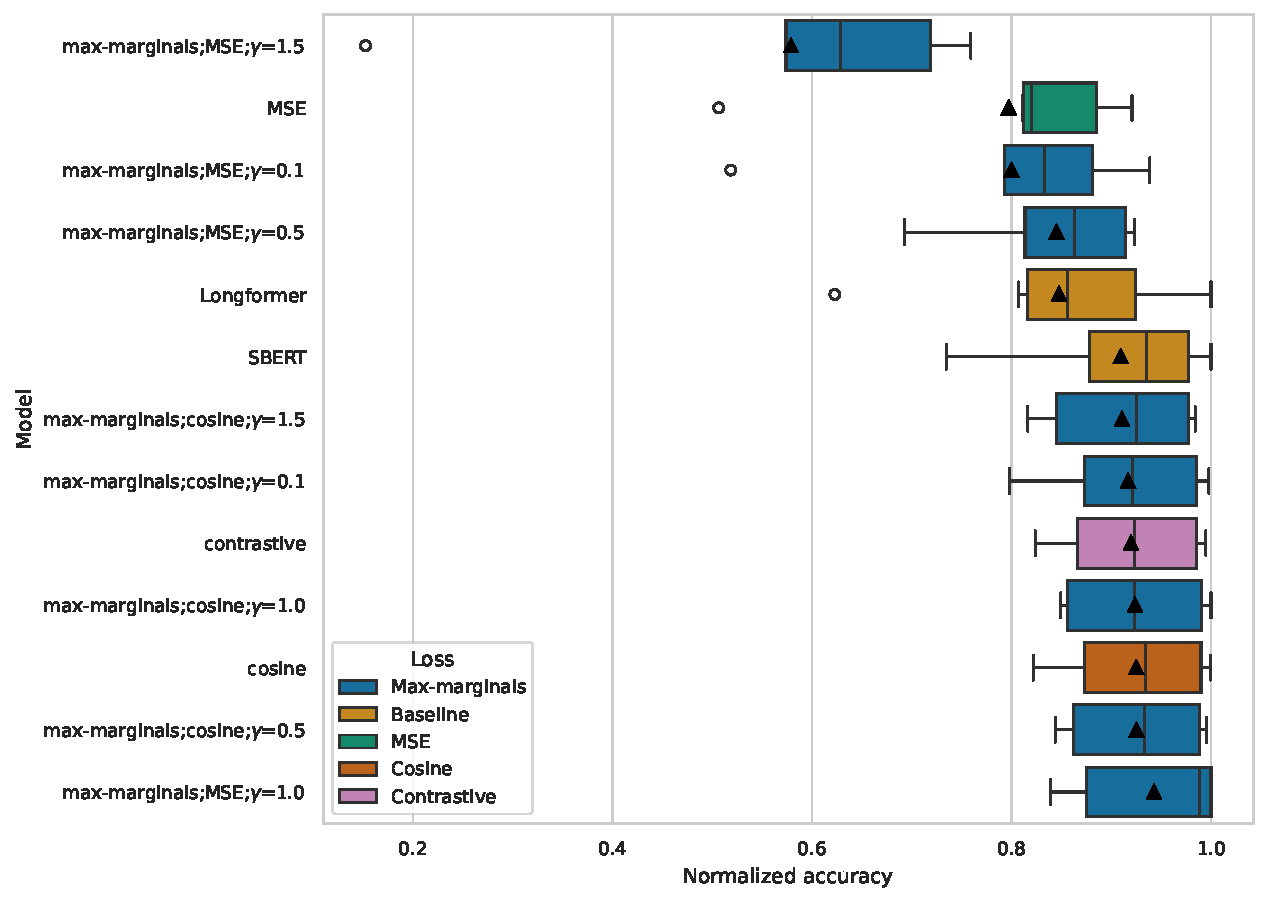
\includegraphics[width=\textwidth]{./img/structural_both_losses.pdf}

  \caption{Comparison of student model performances by loss type.}
  \label{fig:structural_composite_vs_simple}
\end{figure}

\subsubsection{Analysis of composite losses}\label{section:composite_analysis}

The results of composite losses presented in
Figure~\ref{fig:structural_composite_vs_simple} suggest, that the composite
losses using MSE benefit from the negative loss component, whereas the ones
using cosine do not. Furthermore, for most MSE max-marginals losses the benefit
of negative loss component is only marginal. To explain these results we
compare the distances to positives and negatives for several chosen models in
Figure~\ref{fig:composite_distances}. Composite losses using MSE widen the gap
between positive and negative distances at the expense of increasing the
distance to the positives. And so, the benefit of the negative component is not
that it gives a more precise training signal and causes a faster convergence to
the structural teacher's embeddings. Conversely, the benefit comes from a
clearer separation between embeddings of different documents, even if the
generated embeddings do not correspond to the teacher's embeddings that well.
The situation is different for cosine, since its range is limited from the top
and therefore the only option how to increase the gap between the positives and
the negatives is to decrease the distances to the positive. Additionally, all
of the negatives are almost perpendicular to the generated embedding and
therefore direct the generated embedding in only one dimension out of the 768.
Consequently, the benefit of the negative component in cosine composite losses
is very small.

\begin{figure}
  \centering
  \begin{subfigure}{\textwidth}
    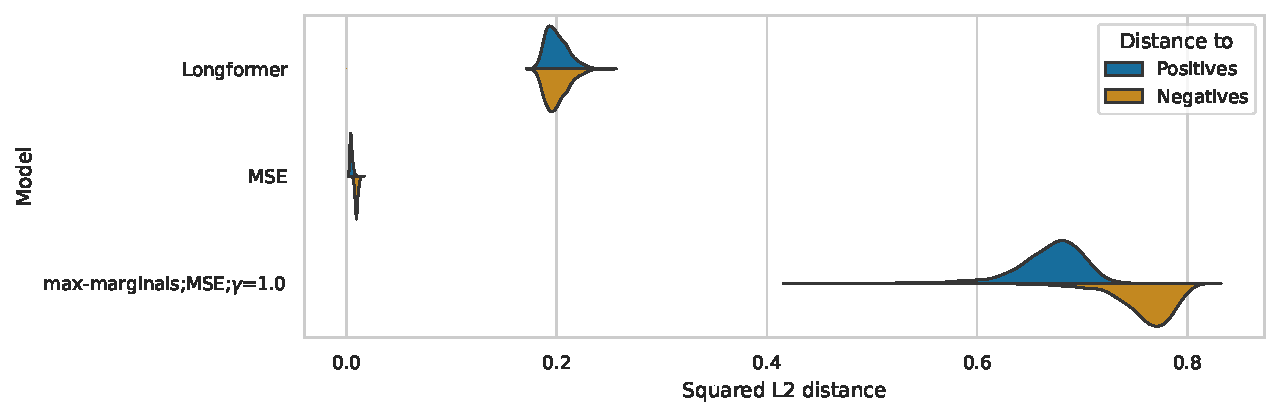
\includegraphics[width=\textwidth]{img/composite_mse_distances.pdf}
    \caption{With MSE}

    \label{fig:composite_mse_distances}

  \end{subfigure}
  \begin{subfigure}{\textwidth}

    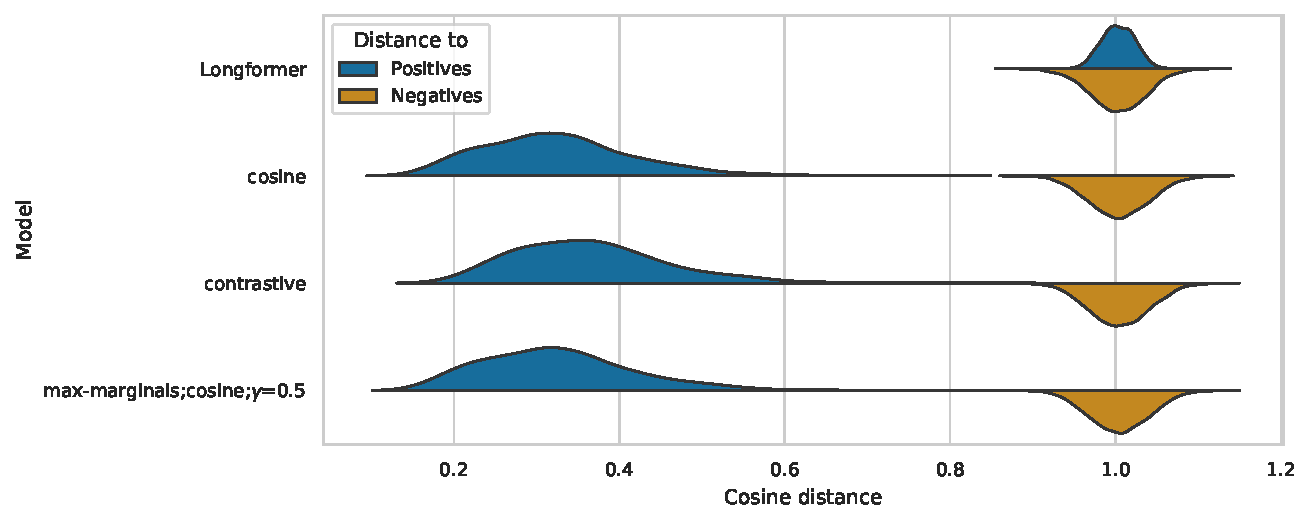
\includegraphics[width=\textwidth]{img/composite_cos_distances.pdf}
    \caption{With cosine}

    \label{fig:composite_cos_distances}
  \end{subfigure}

  \caption{Distribution to distances between the model's and the structural
  teacher's embeddings. A distance to teacher's embedding of the same document
  is labelled as \emph{positive}, whereas distances to teacher's embeddings of
  another document is labelled as \emph{negative}. The distances were generated
  from the first 1000 documents of \Dataset{val\_500k}'s validation split.}

  \label{fig:composite_distances}

\end{figure}

In summary, contrary to our initial hypothesis, the negative loss component
does not ensure faster convergence of the student's embeddings to those of the
structural teacher. In fact, the negative component causes the student's
embedding to move away from the structural teacher's embedding and hence, goes
against the goal of our training. Nonetheless, as we did not want to throw away
a well-performing model and were interested in how the composite loss would
cooperate with a contextual loss, we continue experimenting the best performing
composite loss in the following sections. However, pure cosine loss remains the
preferred structural loss, since it is consistent with the goal of our
training.

\section{Structural and contextual loss}\label{section:improving_both}

In the previous section, we focused on structural losses and found the best
performing one. In this section, we experiment with contextual loss and search
for the one that will complement the already chosen structural loss the best.
We also search for a contextual loss that complements the best performing
composite loss, which we explored in Section~\ref{section:composite_losses}.
Despite contradicting the goal of our training, the max-marginals loss with MSE
outperforms all other structural losses and therefore we continue experimenting
with it in this section.

In Section~\ref{section:paragraph_vector} we explained why we use Paragraph
Vector \citep{le2014distributed} as our contextual teacher. Since there is no
concept of a pre-trained PV, as in the case of transformers, we train PV from
scratch. First, in Section~\ref{section:pv_training} we explore the
hyperparameters of Paragraph Vector's training. Our goal is to find such PV
that will perform the best as a contextual teacher in our teacher-student
training. And so, in Section~\ref{section:contextual_loss}, we pick several PV
models and for each we find the best performing contextual loss given our
structural loss. We also show results of models trained with just the
contextual loss to illustrate how important is structural teacher to the
performance of the student model. Finally, in
Section~\ref{section:weighting_experiments}, we experiment with the weighting
of the two losses for the most promising student models.

\subsection{Optimizing Paragraph Vector's training}\label{section:pv_training}

We do not implement Paragraph Vector, instead we use implementation from Gensim
library\footnote{\label{fn:link_to_gensim}\url{https://radimrehurek.com/gensim}}.
In this section, we explore some of the hyperparameters that govern the
training of PV. From the best performing models, we choose few, which we use as
contextual teachers when experimenting with the contextual loss in the
subsequent section. We focus on four hyperparameters that we consider the most
important, and adopt the recommendation of either the library or related
literature. Both the adopted and the grid-searched hyperparameters are
enumerated in Table~\ref{table:pv_hyperparams}, where the mentioned
hyperparameters have the following meaning:


\begin{itemize}

  \item \texttt{dm} --  PV architecture; true for Distributed Memory (DM),
    false for Distributed Bag of Words (DBOW)

  \item \texttt{vector\_size} -- dimensionality of the generated embedding

  \item \texttt{min\_count} -- words with document frequency below this limit
    will be ignored

  \item \texttt{text\_pre\_process} -- applied word processing done before the
    model's training; for stemming we used PorterStemmer implemented by
    \texttt{nltk}
    library\footnote{\url{https://www.nltk.org/api/nltk.stem.porter.html}}

  \item \texttt{negative} -- number of noise words used for negative sampling
    during training

  \item \texttt{window} -- the maximum distance between known and predicated
    word

  \item \texttt{sample} -- percentile threshold configuring which words will be
    downsampled; 0 for no downsampling


  \item \texttt{dbow\_words} -- whether to train word embeddings using
    Word2Vec \citep{mikolov2013efficient} Skip-gram architecture simultaneously
    with DBOW document embeddings

  \item \texttt{epochs} -- number of iterations over the corpus

\end{itemize}


As recommended by the authors of PV \citep{le2014distributed}, we train
experiment with both architectures. For each architecture we try different
settings of \texttt{vector\_size}, \texttt{min\_count} and
\texttt{text\_pre\_process}, which all control the regularization of the model.
Settings such as higher dimensional embedding, small minimum count and no text
pre-processing, regularize the model the least. They give the model the most
information on its inputs, while also providing it with large embedding through
which the model can express precisely. On the other hand, using lower
dimensional embedding, large minimum count and heavy text pre-processing,
forces the model to be more general and less precise. The model has less
detailed information on its input and must squeeze all of it to a small vector.
We did not see any value in trying dimensions of embeddings higher than 1024 as
in later experiments we need to distill the contextual embedding to a
768-dimensional embedding of our student model. Intuitively, the larger the
contextual embedding is going to be, the smaller the percentage of information
the student model is going to be able to digest. Also there is no value in
considering \texttt{min\_count} to be lower than 2, since we would only add
words that are unique to a single document. Embeddings of such words would be
poorly trained and would not add meaningful information to the document's
embedding. Last hyperparameter that deserves mention is \texttt{dbow\_words}.
DBOW on its own does not train word embeddings, which are randomly generated.
Setting \texttt{dbow\_words} to true causes DBOW to also train word embeddings
using Word2Vec Skip-gram model \citep{mikolov2013efficient} in each epoch.
\cite{lau2016empirical} showed that random word embeddings significantly hurt
the model, and so in our opinion the overall longer training, which training
word embeddings inevitably causes, is worth the performance gain.

\begin{table}
  \footnotesize
  \centering
  \begin{tabular}{lrc}
    \toprule
    Hyperparameter & Value(s) & Recommended by \\
    \midrule
    \texttt{dm} & true, false & - \\
    \texttt{vector\_size} & 100, 768, 1024 & - \\
    \texttt{min\_count} & 2, 10\% of train corpus & - \\
    \texttt{text\_pre\_process} & stem, lowercase, none & - \\
    \texttt{window} & 5 & default \\
    \texttt{negative} & 5 & default, \cite{lau2016empirical} \\
    \texttt{sample} & 0 & default \\
    \texttt{dbow\_words} & true & \cite{lau2016empirical} \\
    \texttt{epochs} & 10 & default, \cite{dai2015document} \\
    \bottomrule
  \end{tabular}

  \caption{Used hyperparameters for training Paragraph Vector. We grid-searched
  four hyperparameters: PV architecture, vector size, minimum word count and
  pre-processing of words. The rest of the hyperparameters we adopted either the
  default values set by the authors of the Gensim
  library\textsuperscript{\ref{fn:link_to_gensim}} or recommended by the
  mentioned literature.}

  \label{table:pv_hyperparams}

\end{table}

We train all variants on \Dataset{val\_500k} corpus. We follow the
recommendations of Paragraph Vector's authors and evaluate also the
concatenation of both architectures. We pick the three best models from each
architecture and we do a cartesian product of the two sets giving us 9 compound
models. In total there are 45 models, whose performance on validation tasks we
report in Figure~\ref{fig:pv_val_scores}. Among the single models, large
embedding dimensions and low minimum count were favored. Additionally, on
average, stemming or lowercasing lead to higher score than not pre-processing
the words at all. DBOWs vary more in performance, occupying the best and the
worst positions, whereas DMs are a bit more consistent. We achieve a slight
improvement by concatenating a DM and a DBOW model, but considering the
resulting model has effectively double the vector size, the improvement is not
surprising. Interestingly, all compound models perform very similarly,
suggesting that slight imperfections of one model can be compensated by another
model of a different architecture.

\begin{figure}

    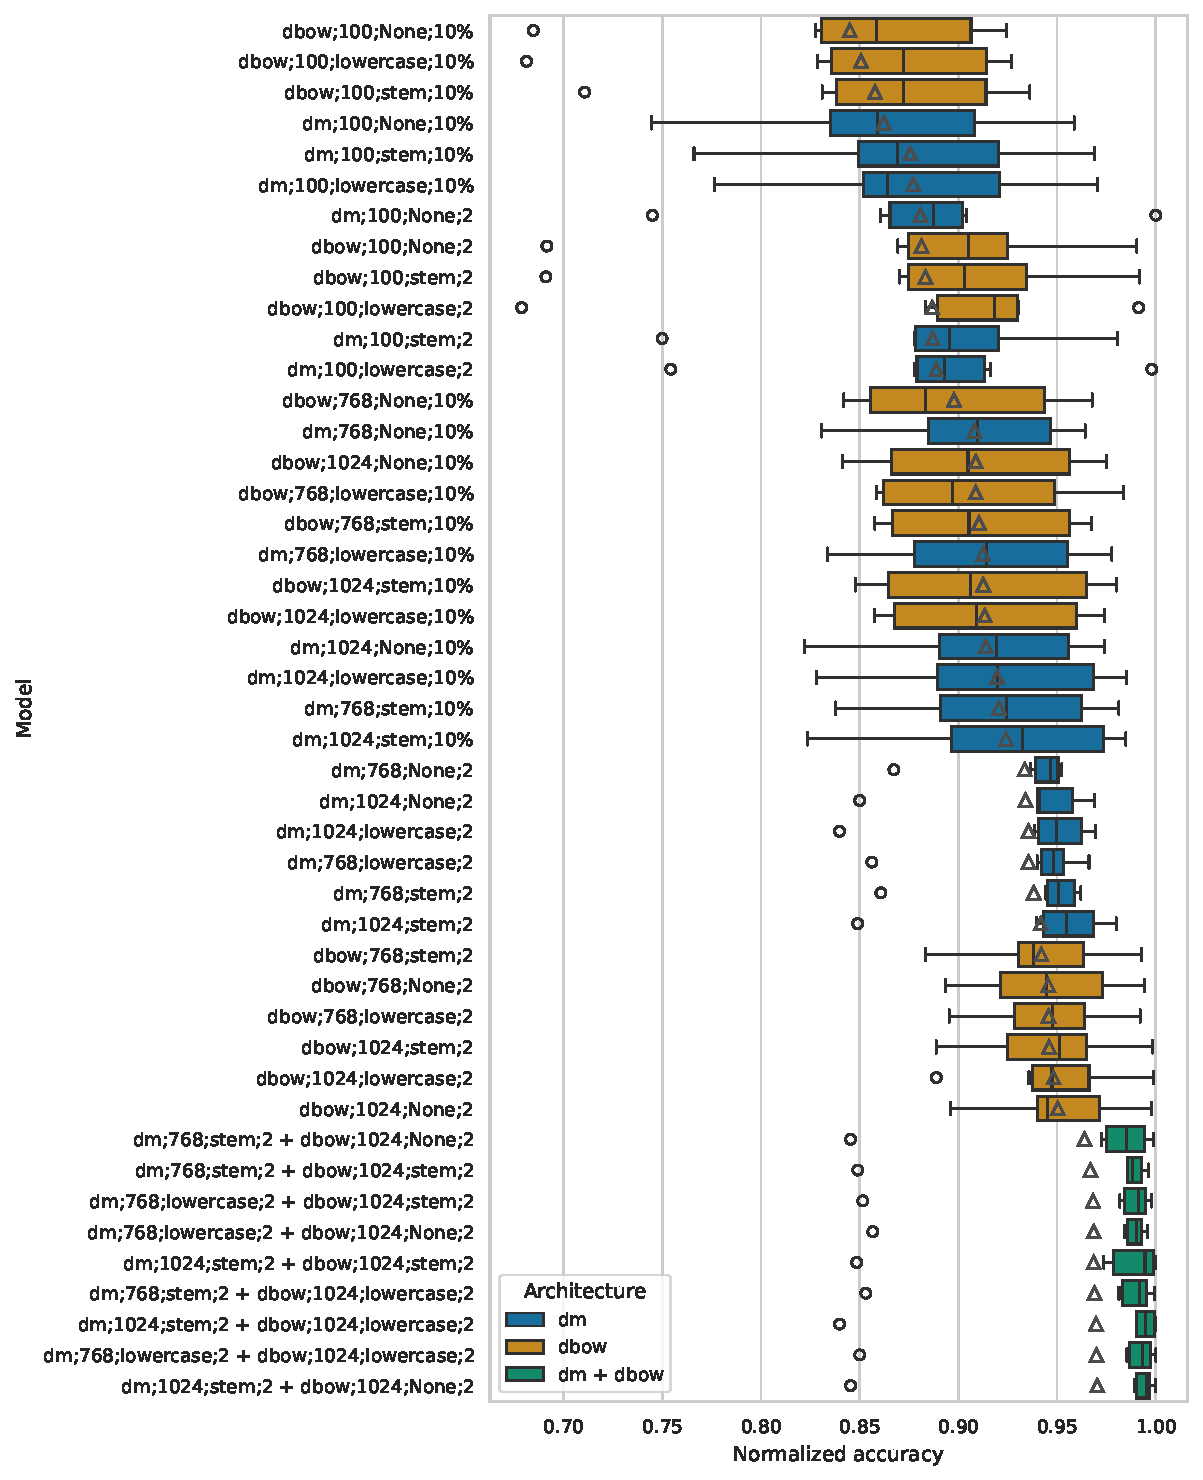
\includegraphics[width=\textwidth]{./img/pv_val_scores.pdf}

    \caption{Performance of all grid-searched Paragraph Vector variants on
    validation tasks. A model is identified by architecture, embedding
    dimension, text pre-processing and minimum count, in this order. Models
    composed of two sub-models are identified as a concatenation of such
    identifiers separated by $+$. The models are sorted according to the mean
    normalized accuracy marked with a triangle.}

    \label{fig:pv_val_scores}

\end{figure}

In our preliminary experiments we saw that the dimension of the contextual
teacher's embedding plays a significant role in the teacher-student training.
And so we select three Paragraph Vectors with varying vector sizes. We pick the
best model with small vector size (\texttt{dm;100;lowercase;2}), the best
single model (\texttt{dbow;1024;None;2}) and the best model composed of both
architectures (\texttt{dm;1024;stem;2 + dbow;1024;None;2}).

% TODO: comparison to longformer, and SBERT
% TODO: label them as DM;100d, DBOW;1024d, PV;2048

\subsection{Contextual loss}\label{section:contextual_loss}

Contextual loss $\Loss_C$ compares the student's and the contextual teacher's
embeddings and encourages distillation of the quality of the teacher's
embedding into the student's embedding. As we discuss in
Section~\ref{section:abstract_loss}, we choose $\Loss_C$ to be less strict and
to give the student model more freedom in how it encodes information in the
document embedding. Consequently we do not consider losses such as MSE, or
cosine, since they enforce either an exact vector or a direction in the
embedding space. Instead we use a variant of \emph{Canonical Correlation
Analysis} \citep{hotelling1992relations} (\emph{CCA}). In its base form CCA
computes a a linear projection, such that the correlation of two sets of
vectors under their individual projections is maximal. We define CCA in
Equation~\ref{def:cca_more_dim}. CCA gives the student the freedom to change
its embeddings as long as their linear projections correlate with the linear
projections of the contextual teacher's embeddings.

\begin{defn}[Canonical Correlation Analysis for more dimensions]\label{def:cca_more_dim}

  For two matrices $X_1 \in \mathbb{R}^{n_1 \times m_1}$ and $X_2 \in
  \mathbb{R}^{n_2 \times m_1}$, Canonical Correlation Analysis for $k$
  dimensions finds $P \in \mathbb{R}^{m_1 \times k}$ and $Q \in \mathbb{R}^{m_2
  \times k}$ that maximize

  \begin{equation}
    \begin{split}
      &\CCA(X_1, X_2) = \sum_{i = 1}^k \corr(X_1P_{*i}, X_2Q_{*i}) \\
      \text{s.t.}\quad &P^TX_1^TX_1P = I_k = Q^TX_2^TX_2Q \\
    \end{split}
  \end{equation}


\end{defn}

However, linear projection may still leave too little leeway for the student
model to simultaneously mimic the structural teacher, while increasing the
correlation with the projected contextual teacher's embeddings. Ideally we
would like to adjust the amount of freedom we give to the student model. Since
CCA does not allow such adjustment, we focus on \emph{Deep CCA} (\emph{DCCA})
\citep{andrew2013deep}. DCCA projects the input vectors with two neural
networks, and then feeds the projections to the vanilla CCA. The two networks
are simultaneously trained together with the embedding model based on the
computed CCA, which is used as a loss. The advantage of DCCA is that we can
adjust the strength of the projections and thereby regulate pressure the
contextual loss inflicts on the student model. The larger the projecting neural
network is, the more it is going to be able to transform the embeddings and the
less the student model is going to need adjust its embedding.

As we can see in Equation~\ref{def:cca_more_dim}, CCA is computed from the
entire dataset of input vectors. And so, DCCA is trained using a full-batch
optimization \citep{andrew2013deep} or a mini-batch optimization with large
batch sizes \citep{wang2015unsupervised}. However, both methods need large
amount of GPU memory and therefore are applicable only to small models. For
this reason we avoid DCCA and use SoftCCA \citep{chang2018scalable}, which
reformulates CCA, such that it is usable even in case of mini-batch
optimization with small batches. To explain how SoftCCA is related to CCA we
reformulate the solution of CCA using a Forbenious matrix norm in
Equations~\ref{def:cca_with_forbenious_first}-\ref{def:cca_with_forbenious_last}.

\begin{align}
  P^\ast, Q^\ast &= \underset{P, Q}{\argmin} ||X_1P - X_2Q||^2_F \label{def:cca_with_forbenious_first} \\
  &= \underset{P, Q}{\argmin} \trace\left((X_1P - X_2Q)^T(X_1P - X_2Q)\right) \\
  &= \underset{P, Q}{\argmin} {-2} \trace(P^TX_1^TX_2Q) \\
  &= \underset{P, Q}{\argmax} \trace(P^TX_1^TX_2Q) \\
  &= \underset{P, Q}{\argmax} \sum_{i = 1}^k \corr(X_1P_{*i}, X_2Q_{*i}) \label{def:cca_with_forbenious_last}
\end{align}

Thus, by minimizing CCA we effectively minimize the difference between two
projections with uncorrelated features. SoftCCA mimics these two effects with
two separate losses:

\begin{itemize}

  \item L2 loss which minimizes of the difference between projections:

    \begin{equation}
      \Loss_{\text{L2}}(X_1, X_2) = ||X_1 - X_2||^2_F = \MSE(X_1, X_2)
    \end{equation}

  \item \emph{Soft Decorrelation Loss} (\emph{SDL}) which forces a projection
    to have decorrelated features:

    \begin{equation}
      \Loss_{\text{SDL}}(X^t) = \sum_{i \ne j} \left|
          \frac{(\Phi^t_X)_{ij}}{\hat{\beta}^t}
          \right|
    \end{equation}
    where
    \begin{align}
      \Phi^t_X &= \beta \Phi^{t-1}_X + \Sigma_{X^t} \\
      \Phi^0_X &= \bm{0}_d \\
      \hat{\beta}^t &= \beta \hat{\beta}^{t-1} + 1 \\
      \hat{\beta}^0 &= 0
    \end{align}

\end{itemize}

Where

\begin{itemize}

  \item $X, X_1, X_2 \in \mathbb{R}^{b \times d}$ are mini-batches of
    $d$-dimensional vectors

  \item $\Sigma_{X}$ is a covariance matrix of a mini-batch of vectors $X$

  \item $\bm{0}_d$ is a $d \times d$ zero matrix

  \item $\beta$ is a hyperparameter

  \item $\Phi_X^t, X^t, \hat{\beta}^t$ is $\Phi_X, X, \hat{\beta}$ at iteration
    $t$

\end{itemize}

The L2 loss forces the projected vectors to be equal, while the Soft
Decorrelation Loss forces them to have uncorrelated features. Notice that to
have a better estimate of the projected vector's covariance matrix, SDL keeps a
running mean. Similarly to Batch Normalization \citep{ioffe2015batch}, SDL
updates the running mean during training, but avoids any updates during
inference. With the above losses, and the weighting hyperparameter
$\delta$, we define SoftCCA in Equation~\ref{eq:soft_cca}.

\begin{equation}\label{eq:soft_cca}
  \Loss_{\text{SoftCCA}}(X_1, X_2) = \Loss_{\text{L2}}(X_1, X_2) +
      \delta ( \Loss_{\text{SDL}}(X_1) + \Loss_{\text{SDL}}(X_2) )
\end{equation}

We use SoftCCA loss as a replacement for CCA in DCCA. To be explicit, we
project the student's and the contextual teacher's embedding with two separate
feed-forward neural networks and then apply SoftCCA loss, which provides
training signal not only for the embedding model, but also for the neural
networks projecting the embeddings. For brevity we call the neural networks
that project the student's and the contextual teacher's embedding
\emph{student} and \emph{contextual projections}, respectively. We illustrate
the used contextual loss graphically in Figure~ref{} (TODO: image).

In our preliminary experiments, we found that the value of $\delta$ makes
little difference and so we set it so that the ranges of $\Loss_{\text{L2}}$
and $\Loss_{\text{SDL}}$ are roughly equal. On the other hand, choosing a
correct value of $\beta$ showed to be critical. Based on how the CCA of the
projected embeddings of the validation split progressed throughout the
training, we found the optimal value to be 0.95, which puts relatively large
emphasis on the accumulated mean compared to lower values of $\beta$.

In the rest of this section, we experiment with the strength of the
projections. In the following section we build the basic intuition behind
training with the two projections and SoftCCA, while finding the ideal
contextual projection without any structural loss. In the subsequent sections
we study how different structural losses influence the ideal projection. First
we experiment with cosine and then with max-marginals MSE loss. In all cases we
test the projections for each of the three contextual teachers we selected in
previous section. At the end, we select the best contextual loss with the best
contextual teacher for both cosine and max-marginals MSE structural loss, with
which we experiment further later in this chapter.

\subsubsection{Contextual projection with contextual loss
only}\label{section:projections_only_contextual}

With only the contextual loss, the student's only goal is to mimic the
contextual teacher's embedding. This presents a very basic setting, in which we
can study the behaviour of the projections and of the contextual loss as a
whole without any influence from the structural loss.

As we learned in our preliminary experiments over parameterization of the
projections hurts the performance of the model. Even though large projections
result in smaller SoftCCA loss, they tend to harm the CCA of the student's and
contextual teacher's embeddings. Strong projections compensate for the
student's flaws, which lessens the pressure on the student model as it does not
need to adjust its embedding that much. As a consequence, the student model
learns very little compared to the projections. Similarly, strong contextual
projections can take away pressure from the student projection and
vice-versa. In this regard, it is important to keep the contextual projection
small, to put more pressure on the student's side where the gradients can
propagate to the embedding model itself.

% TODO: bottle-neck like architectures do not do well

As we mentioned before, we feed the projected outputs to SoftCCA loss
$\Loss_{\text{SoftCCA}}$. As SoftCCA requires both inputs to be of the same
dimension, both projections must end with an equally sized layer. We always use
the dimension of the larger embedding as the final projection dimension. We do
so, to preserve all information contained in a embedding through the
projection. With even larger final projection dimension, some of the final
vector's features would have to rely on the same embedding's features due to
the Pigeonhole principle. Consequently some of the final features would be
inevitably correlated. This would create unnecessary conflict with the SDL
loss, which forces the projections to output uncorrelated features.

We build the projections as a sequence of blocks, where each block is composed
of a fully connected layer and a optional Rectified Linear Unit (\emph{ReLU}).
In preliminary experiments, we also tried adding Dropout, Batch or Layer
Normalization layers at different places in a block, but they have either
negligible or negative effect on the performance of the final model. We label
each block with the dimension of the fully connected layer and with the
activation's name in brackets if it is used. The whole projection is then
identified by block's labels delimited by an ``x''. So, \Proj{768(ReLU)x1024}
are two feed forward layers with 768 and 1024 features connected via ReLU. To
label projections without any layers we use a dash. We present all the
projections' variations we tested in Table~\ref{table:contextual_projections}.

% TODO: briefly how we picked the variants

\begin{table}
  \centering
  \footnotesize

  \begin{tabular}{lrrr}
    \toprule
      & \multicolumn{3}{c}{Contextual teacher's embedding dimension} \\
      \cline{2-4} \\
      Projection & 100 & 1024 & 2048 \\
    \midrule
      \multirow[t]{2}*{Student} & \Proj{768(ReLU)x1024(ReLU)x768} & \Proj{768(ReLU)x1024} & \Proj{1024(ReLU)x2048} \\
      & \Proj{768} & \Proj{1024} & \Proj{2048} \\
      \multirow[t]{3}*{Contextual} & \Proj{100(ReLU)x768} & \Proj{768x1024} & \Proj{1024x2048} \\
      & \Proj{768} & \Proj{1024} & \Proj{2048} \\
      & & - & - \\
    \bottomrule
  \end{tabular}

  \caption{All tested variants of projections with only contextual loss. We do
  a grid search of the given variants for each contextual teacher. This results
  in 16 student models overall.}

  \label{table:contextual_projections}
\end{table}

We train the student models on the first 15k documents of \Dataset{val\_500k}.
We compare the models' performance to all the relevant
teachers, Longformer and the best structural model in
Figure~\ref{fig:projections_contextual}. The results correspond to those we
witnessed in our preliminary experiments and confirm the discussion from
previous paragraphs. The better half of the student models differed from the
rest by having a minimal contextual projection. Moreover, for a given
contextual teacher and projection, the student model with larger student
projection outperforms the student with a smaller one in all cases except for
one.

Half of the tested projections improve the score of Longformer, suggesting that
we are able to distill useful information from the contextual teacher to the
student. However, as our contextual loss does not enforce exact similarity of
the student's and the contextual teacher's embedding, most of the students do
not outperform their respective contextual teachers. Interestingly, students
trained with contextual embeddings with 100 dimensions surpass students trained
with better performing 1024-dimensional contextual embeddings. The same can be
said for 1024 and 2048 dimensional embeddings, even when comparing projections
that increase with the size of the contextual teacher's embeddings, such as
\Proj{1024d;S:1024;C:-} and \Proj{2048d;S:2048;C:-} or
\Proj{1024d;S:1024;C:1024} and \Proj{2048d;S:2048;C:2048}. Consequently, it
seems that it is easier to distill information from an embedding with less
features than from a larger one. As a consequence, even though PV with 2048
dimensions beats SBERT, the students trained with it fail to capitalize on this
advantage and perform worse than the model trained with SBERT. And so in our
experiments the structural teacher is more important to the student's
performance than the contextual teacher and justifies why we search for the
ideal contextual loss to the best performing structural loss rather than the
other way around.

\begin{figure}

  \centering

  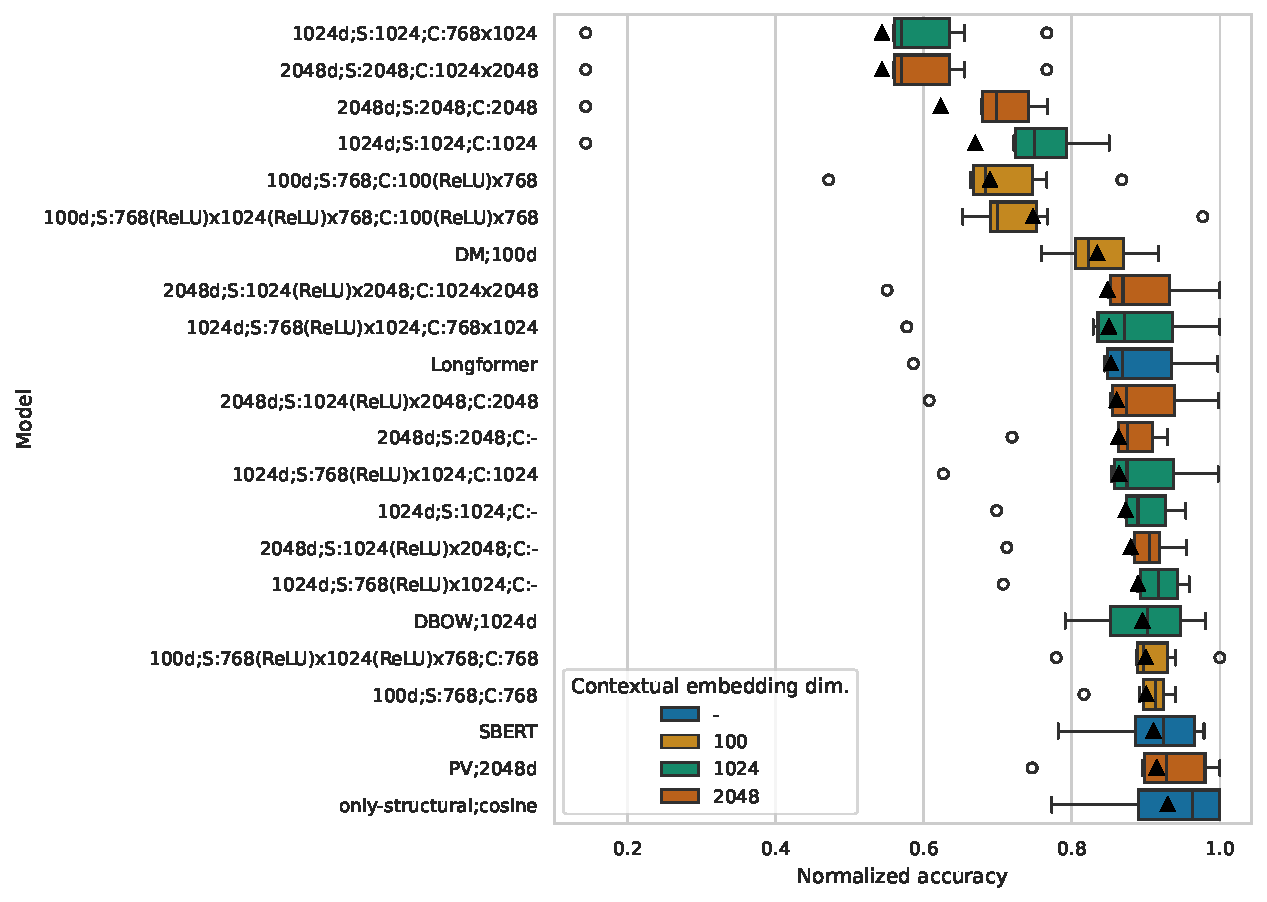
\includegraphics[width=\textwidth]{img/projections_contextual.pdf}

  \caption{Performances of student models trained with only the contextual
  loss. We compare the students to all the relevant teachers, Longformer and
  the best student model trained with only the structural loss. We identify
  students trained with just the contextual loss with the contextual embedding
  dimension, student and contextual projection, in this order.}

  \label{fig:projections_contextual}

\end{figure}

\subsubsection{Contextual projection with cosine structural loss}

We now search for the best performing projections while simultaneously using
cosine structural loss. Compared to the previous section, the training is a bit
more complex as the student is now forced to distill two qualities, each from a
different teacher. So, even though the student and contextual
projections still behave in the same manner, they may cause different outcomes.

We list all the tested projections in
Table~\ref{table:cos_contextual_projections}. We added stronger projections,
while discarding some of the less successful projections from the previous
section. We again train the student models on the first 15k documents of
\Dataset{val\_500k} and present the performance of the trained student models
in Figure~\ref{fig:cos_projections_contextual}. Compared to the student models
trained with just the contextual loss, the same projection variants differ less
with the cosine structural loss. By using the cosine structural loss, all of
the student models get a performance boost that seems to lessen the negative
effect of bad performing projections. As a consequence, almost all of the
student models surpass all baselines. The best performing projections are much
larger compared to the best projections trained without any structural loss. It
seems that as we increase the pressure on the student by adding a structural
loss, we need to simultaneously give the model more freedom on the side of the
contextual loss. With the larger projections we were able to surpass the best
student model trained with just the structural loss. This shows that, with well
performing projections, the student model benefits from the fact that both
losses are being used during training. Even if the performance gain is not
huge, we can say the contextual and structural embeddings complement each
other.

\begin{table}
  \centering
  \footnotesize

  \begin{subtable}{\textwidth}
    \centering
    \begin{tabular}{lr}
      \toprule
        & Contextual teacher's embedding dimension \\
        \cline{2-2} \\
        Projection & 100 \\
      \midrule
        Student & \Proj{768(ReLU)x1024(ReLU)x768}  \\
        \multirow[t]{2}*{Contextual} & \Proj{100(ReLU)x768}  \\
        & \Proj{768} \\
      \bottomrule
    \end{tabular}
    \caption{100 dimensional contextual teacher}
  \end{subtable}
  \medskip

  \begin{subtable}{\textwidth}
    \centering
    \begin{tabular}{lrr}
      \toprule
        & \multicolumn{2}{c}{Contextual teacher's embedding dimension} \\
        \cline{2-3} \\
        Projection & 1024 & 2048 \\
      \midrule
        Student &  \Proj{768(ReLU)x1024} & \Proj{1024(ReLU)x2048} \\
        \multirow[t]{2}*{Contextual} &  \Proj{1024} & \Proj{2048} \\
        & - & - \\
      \midrule
        Student & \Proj{768(ReLU)x4096(ReLU)x1024} & \Proj{768(ReLU)x4096(ReLU)x2048} \\
        \multirow[t]{3}*{Contextual} & \Proj{768(ReLU)x1024} & \Proj{2048(ReLU)x2048} \\
        & \Proj{1024} & \Proj{2048} \\
        & - & - \\
      \bottomrule
    \end{tabular}

    \caption{1024 and 2048 dimensional contextual teachers}

  \end{subtable}

  \caption{All tested variants of projections with contextual loss and cosine
  structural loss. For a given contextual teacher, we delimit each group of
  projections by a horizontal line. We grid search all variants within a
  projections group. This gives 12 student models in total.}

  \label{table:cos_contextual_projections}
\end{table}

\begin{figure}

  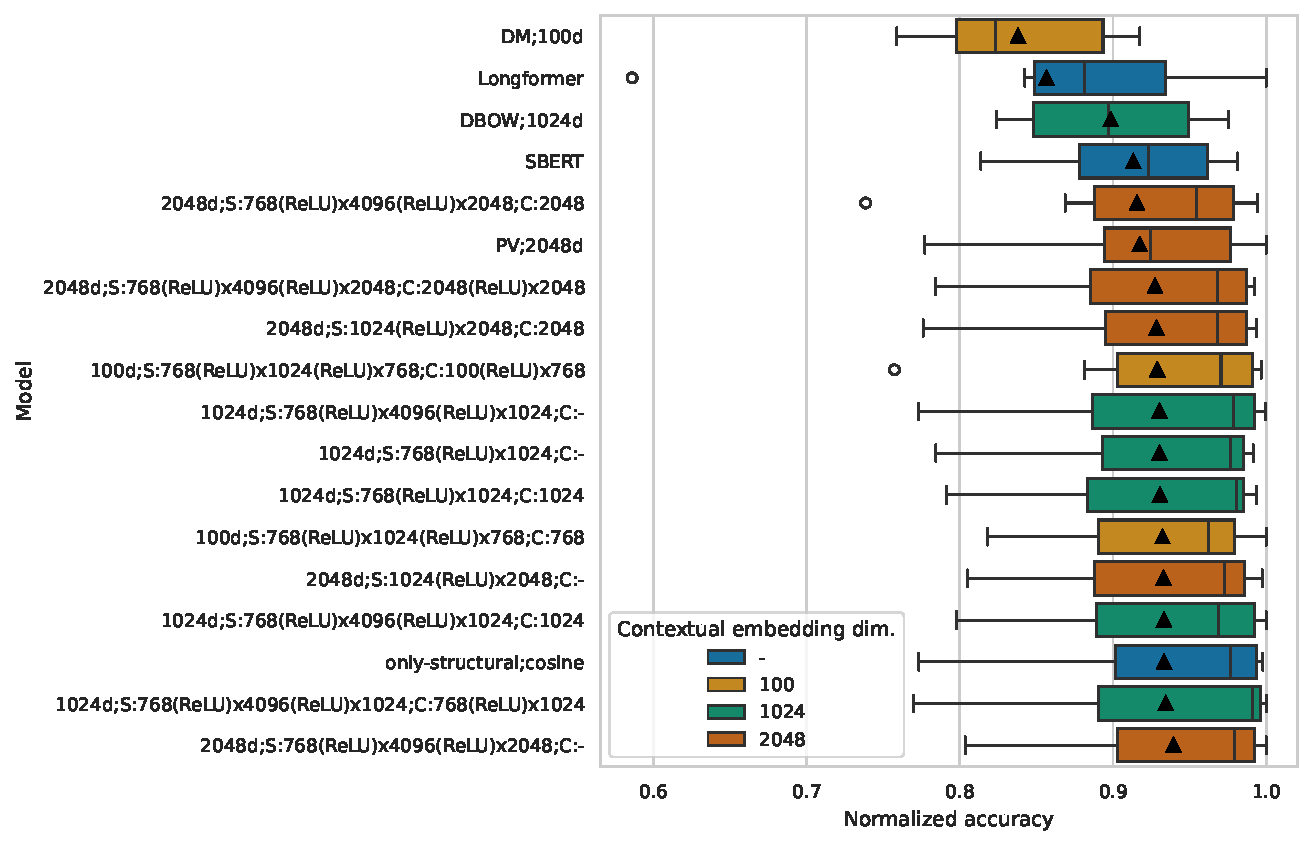
\includegraphics[width=\textwidth]{img/projections_contextual_cos.pdf}

  \caption{Performance of student models trained with contextual and cosine
  structural loss on validation tasks. We compare the student models to all
  relevant teachers, Longformer and the best student model trained with just
  the structural loss.}

  % TODO: Longformer is better 'base student checkpoint' -- Just say what is
  % the base student checkpoint and then use the name that was already given to
  % it by the authors - Longformer.

  \label{fig:cos_projections_contextual}

\end{figure}

\subsubsection{Contextual projection with max-marginals MSE structural loss}

We also search for the optimal projections when training with the max-marginals
MSE loss. Although, as we show in Section~\ref{section:composite_analysis},
max-marginals MSE structural loss goes against the goal of our student-teacher
training, it performed the best out of all composite and simple structural
losses. We continue experimenting with it here, to see how does the student
react if we also include the contextual loss.

We present all the tested projection variants in
Table~\ref{table:mm_mse_contextual_projections}. We included successful
projections from previous section and add stronger contextual projections as
they perform surprisingly well with max-marginals MSE structural loss. Same as
in the previous two sections, we train all student models on the first 15k
documents from \Dataset{val\_500k} and compare their performance to all
relevant teachers, Longformer and the student model trained with just the given
structural loss. We present the model's performances in
Figure~\ref{fig:mm_mse_contextual_projections}. As is the case with the cosine
structural loss, max-marginals MSE loss also boosts the students' performances.
Again, as a consequence, we see that the student's performances are not as
dependent on the projections as is the case of students trained without any
structural loss. Contrary to what we witness in previous experiments, stronger
contextual projections perform overall very well. Even if the best two models
have weaker contextual projections, the majority of the above average student
models, projects the contextual teacher's embedding with two layers. Whereas
the majority of the below average student models, has one or no contextual
layers. This suggests that max-marginals MSE exerts so much pressure on the
student's embedding, that the contextual projection needs to be strong enough
to conform to it. However, based on the two best performing projections, we see
that an even larger student projection might compensate for a small contextual
projection. Nonetheless, max-marginals MSE loss is so strict, it is more
difficult to design the contextual loss so that the student benefits from it
being used along the structural loss.

\begin{table}
  \centering
  \footnotesize

  \begin{subtable}{\textwidth}
    \centering
    \begin{tabular}{lr}
      \toprule
      % TODO: name the same in the chart or rename it here
        & Contextual teacher's embedding dimension \\
        \cline{2-2} \\
        Projection & 100 \\
      \midrule
        \multirow[t]{2}*{Student} & \Proj{768(ReLU)x1024(ReLU)x768}  \\
        & \Proj{768} \\
        \multirow[t]{2}*{Contextual} & \Proj{100(ReLU)x768}  \\
        & \Proj{768} \\
      \bottomrule
    \end{tabular}
    \caption{100 dimensional contextual teacher}
  \end{subtable}
  \medskip

  \begin{subtable}{\textwidth}
    \centering
    \begin{tabular}{lrr}
      \toprule
        & \multicolumn{2}{c}{Contextual teacher's embedding dimension} \\
        \cline{2-3} \\
        Projection & 1024 & 2048 \\
      \midrule
        Student &  \Proj{768(ReLU)x1024} & \Proj{1024(ReLU)x2048} \\
        \multirow[t]{3}*{Contextual} & \Proj{768x1024} & \Proj{1024x2048} \\
        & \Proj{1024} & \Proj{2048} \\
        & - & - \\
      \midrule
        Student & \Proj{768(ReLU)x4096(ReLU)x1024} & \Proj{768(ReLU)x4096(ReLU)x2048} \\
        \multirow[t]{3}*{Contextual} & \Proj{1024(ReLU)x1024} & \Proj{2048(ReLU)x2048} \\
        & \Proj{768(ReLU)x1024} & - \\
      \bottomrule
    \end{tabular}

    \caption{1024 and 2048 dimensional contextual teachers}

  \end{subtable}

  \caption{All tested variants of projections with contextual loss and
  max-marginals MSE structural loss. For a given contextual teacher, we delimit
  each group of projections by a horizontal line. We grid search all variants
  within a projections group. This gives 14 student models in total.}

  \label{table:mm_mse_contextual_projections}
\end{table}

\begin{figure}

  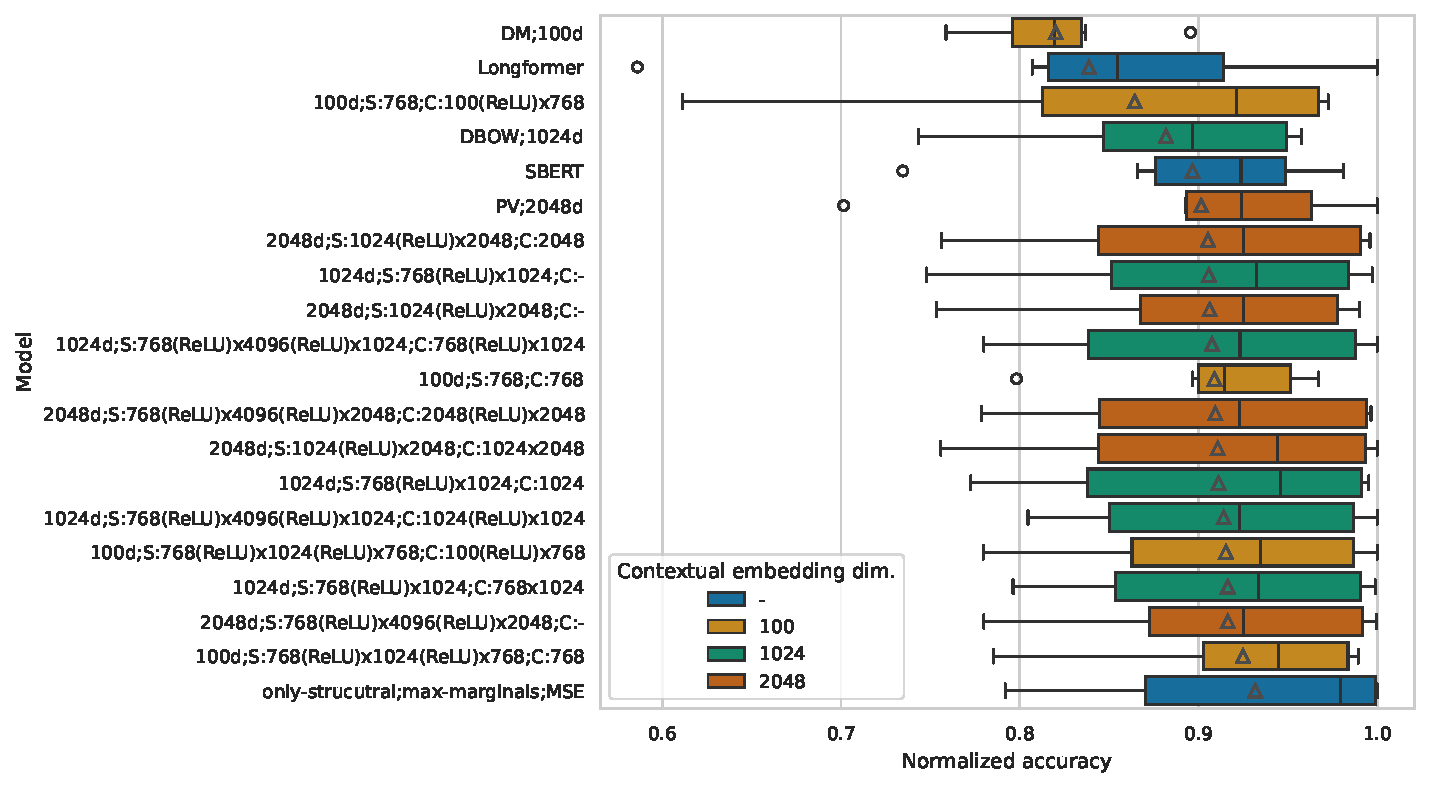
\includegraphics[width=\textwidth]{img/projections_contextual_mm_mse.pdf}

  \caption{Performance of student models trained with contextual and
  max-marginals MSE structural loss on validation tasks. We compare the student
  models to all relevant teachers, Longformer and the student model
  trained with just the max-marginals MSE structural loss.}

  \label{fig:mm_mse_contextual_projections}

\end{figure}

\subsection{Weighting of structural and contextual
loss}\label{section:weighting_experiments}

The final loss is a weighted sum of the contextual and the structural loss. In
this section we explore two weighting mechanisms. First, we assign static
weights to each loss. Second, we combine the static weights with dynamic
masking of inputs based on their length. As the structural teacher has limited
context length, its embedding only reflects the information in the first 384
tokens. We use dynamic masking to train the student only on those inputs, which
the structural teacher encoded whole. Therefore, in theory, the structural loss
should be more reliable. To summarize, there are two parameters which we grid
search: \texttt{max\_structural\_len} and $\lambda$.
\texttt{max\_structural\_len} determines which inputs' structural loss we
mask-out. $\lambda$ is the static weight that is used for unmasked inputs to
balance the importance of structural and contextual loss. For clarity, we
include a Python-like pseudocode of the weighting algorithm:

\bigskip
\begin{lstlisting}
length_mask @\High{symbols}=@ torch.@\High{functions}ones@(batch_size)
if max_structural_len is not @\High{types}None\High{symbols}:@
  length_mask @\High{symbols}=@ lengths @\High{symbols}<=@ max_structural_len
lams @\High{symbols}=@ torch.@\High{functions}zeros@(batch_size).@\High{functions}fill\verb|_|@(@$\lambda$@)
lams @\High{symbols}*=@ length_mask

# For each loss we expect shape (batch_size,)
structural_loss @\High{symbols}=@ ...
contextual_loss @\High{symbols}=@ ...

loss @\High{symbols}=@ structural_loss @\High{symbols}*@ lams @\High{symbols}+@ contextual_loss @\High{symbols}*@ (@\High{constants}1@ @\High{symbols}-@ lams)
loss @\High{symbols}=@ torch.@\High{functions}mean@(loss)
\end{lstlisting}
\bigskip

We consider two structural losses: cosine and max-marginals MSE. For each
structural loss we take the two best-performing contextual losses from the
previous section and try all combinations of hyperparameters' values we list in
Table~\ref{table:weighting_variants}.

\begin{table}
  \centering
  \footnotesize
  \begin{tabular}{cc}
    \toprule
    \texttt{max\_structural\_len} & $\lambda$ \\
    \midrule
    384 & 0.95 \\
    None & 0.8 \\
    & 0.5 \\
    & 0.2 \\
    \bottomrule
  \end{tabular}

  \caption{Tested weighting hyperparameters' values. We experiment with several
  static weightings of the two losses combined with or without dynamic masking
  of structural losses for inputs longer than 385 tokens.}

  \label{table:weighting_variants}

\end{table}

\subsubsection{Weighting a contextual and the cosine structural loss}

\begin{figure}

  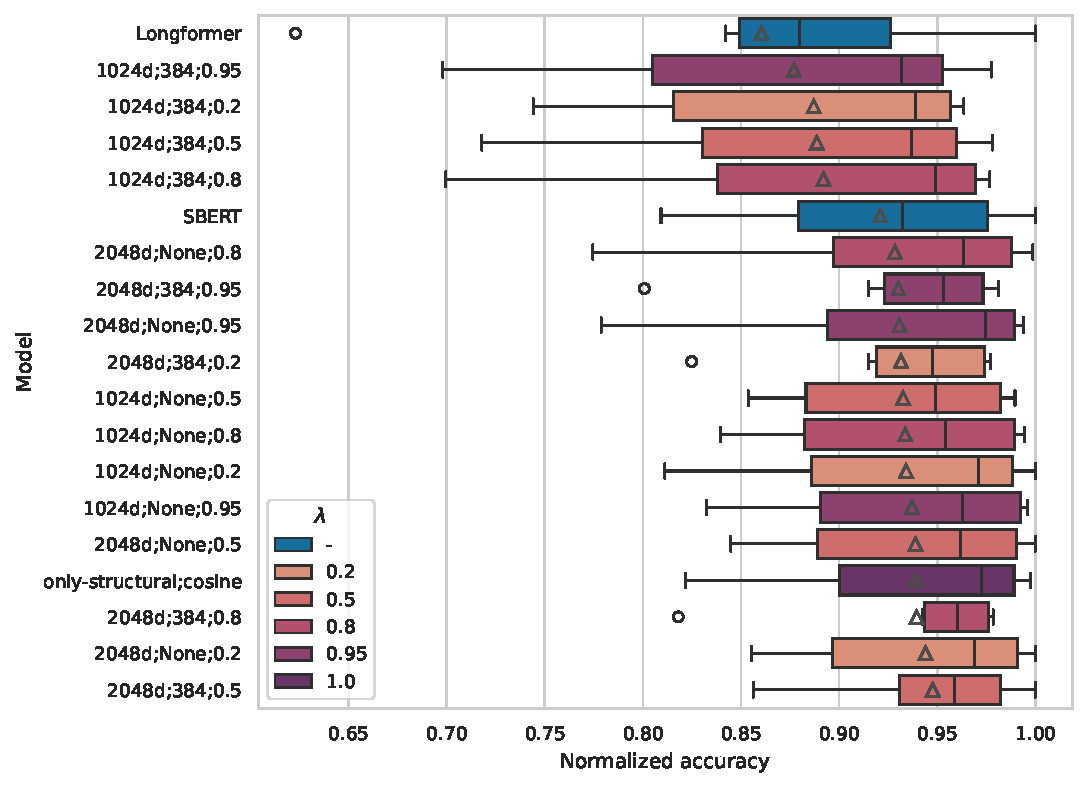
\includegraphics[width=\textwidth]{img/cos_weighting.pdf}

\end{figure}

\subsubsection{Weighting a contextual and the max-marginals MSE structural
loss}

\begin{figure}

  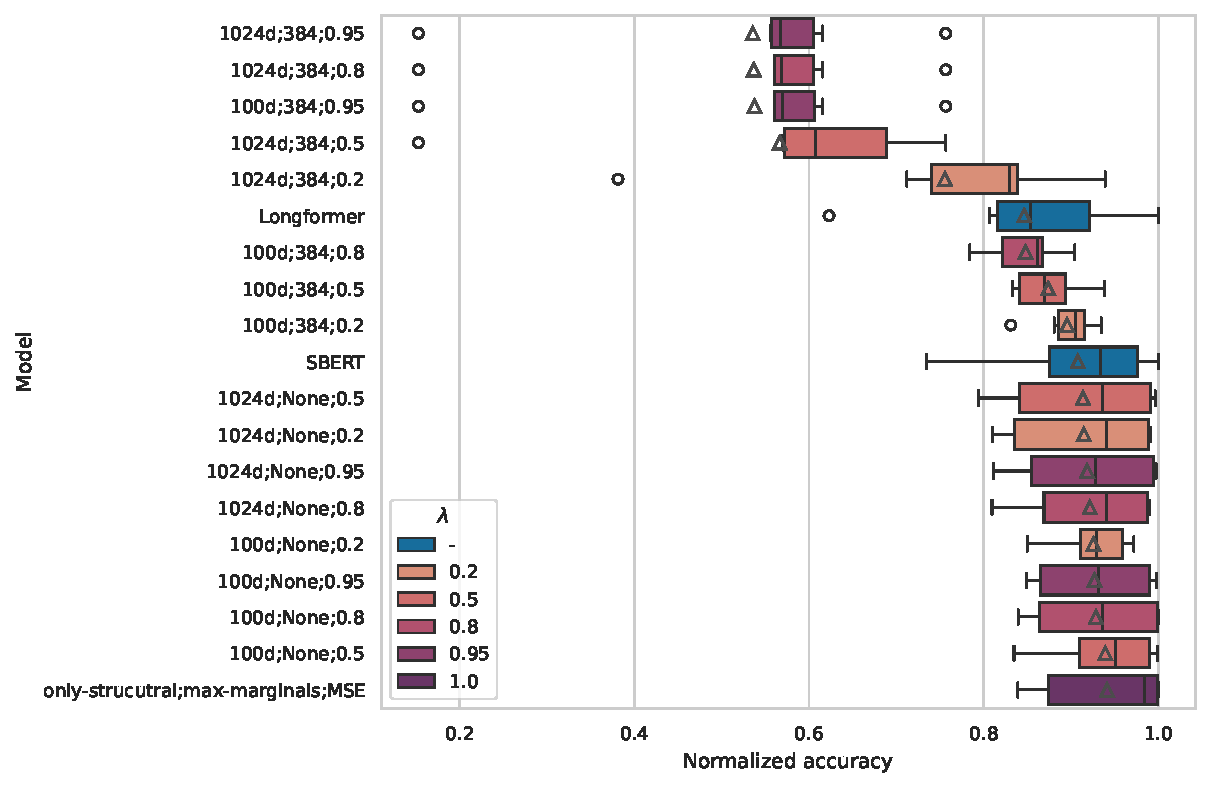
\includegraphics[width=\textwidth]{img/mm_mse_weighting.pdf}

\end{figure}
